\documentclass[titlepage]{book}

% Packages
\usepackage[fontsize=12pt]{fontsize}
\usepackage[utf8]{inputenc}
\usepackage{afterpage}
\usepackage{chngcntr}
\usepackage{blindtext}
\usepackage[TS1,T1]{fontenc}
\usepackage[english]{babel}
\usepackage{tikz}
\usepackage[title]{appendix}
\usepackage{graphicx}
\usepackage{graphbox}
\usepackage{enumitem}
\usepackage{fancyhdr}
\usepackage[margin=2cm, bottom = 6.5em]{geometry}
\usepackage{gensymb}
\usepackage{xcolor}
\usepackage{amsmath}
\usepackage{amsthm}
\usepackage{amssymb}
\usepackage{dsfont}
\usepackage{mathrsfs}
\usepackage[hyperfootnotes = false , linktoc = page, pdfpagelayout = TwoPageRight]{hyperref}
\usepackage{comment}
\usepackage{lettrine}
\usepackage{cfr-lm}
\usepackage{makecell}
\usepackage{soul}
\usepackage{mathtools}
\usepackage{booktabs}
\usepackage{subcaption}
\usepackage{natbib}
\usepackage{apalike}
\usepackage{xassoccnt}
\usepackage{array}
\usepackage[labelsep = space]{caption}
\usepackage[singlespacing]{setspace}
\usepackage[flushmargin,multiple]{footmisc}
\usepackage{multicol}
\usepackage[defaultlines=4,all]{nowidow}
\usepackage{titlesec}
\usepackage{tocloft}
\usepackage{wrapfig}
\usepackage{multirow}

\DeclareMathOperator*{\argmax}{arg\,max}
\DeclareMathOperator*{\argmin}{arg\,min}
\setlength{\parindent}{0em}
\setlength{\parskip}{1em}
\renewcommand{\baselinestretch}{1}
\newenvironment{thisnote}{\par\color{blue}}{\par}
\makeatletter
\def\FN@baselinestretch{.6}
\makeatother
\renewcommand\qedsymbol{$\blacksquare$}
\newenvironment{solution}
 {\renewcommand\qedsymbol{$\blacksquare$}\begin{proof}[Solution]}
 {\end{proof}}
\newcommand{\dd}{\text{ d}}
\newcommand{\E}[1]{\mathbb{E}\left[#1\right]}
\newcommand{\Ex}[2]{\mathbb{E}_{#1}\left[#2\right]}
\newcommand{\Var}[1]{\text{Var}\left(#1\right)}
\newcommand{\Cov}[1]{\text{Cov}\left(#1\right)}
\newcommand{\pr}[1]{\text{Pr}\left(#1\right)}
\newcommand{\PP}[1]{\mathbb{P}\left[#1\right]}
\newcommand{\pto}{\overset{p}{\to}}
\newcommand{\dto}{\overset{d}{\to}}
\newcommand{\Perp}{\perp\!\!\!\perp}

\bibliographystyle{apalike}


\newcommand{\foo}{\makebox[0pt]{\textbullet}\hskip-0.5pt\vrule width 1pt\hspace{\labelsep}}

\def\citeapa #1{\citeauthor{#1}, \citeyear{#1}}

\hypersetup{
    colorlinks,
    linkcolor={red!100!black},
    citecolor={blue!100!black},
    urlcolor={blue!100!black}
}

\theoremstyle{plain}
\newtheorem{thm}{Theorem}[subsection]
\newtheorem{lem}[thm]{Lemma}
\newtheorem{prop}[thm]{Proposition}
\newtheorem*{cor}{Corollary}

\theoremstyle{definition}
\newtheorem{defn}{Definition}[subsection]
\newtheorem{conj}{Conjecture}[section]
\newtheorem{exmp}{Example}[subsection]

\theoremstyle{remark}
\newtheorem*{rem}{Remark}
\newtheorem*{note}{Note}

\DeclareCoupledCountersGroup{thms}
\DeclareCoupledCounters[name=thms]{thm, defn, exmp}

% For tables - From Kenneth's Automata and Bayesian Updating
\tikzstyle{rect}=[rectangle, rounded corners, fill=white!20, text centered, draw=black,  minimum height=1.7em]
\tikzstyle{rectb}=[rectangle, rounded corners, fill=white!20, text centered, draw=blue,  minimum height=1.7em]

% Two node styles: solid and hollow - for game trees
\tikzstyle{solid node}=[circle,draw,inner sep=1.2,fill=black]
\tikzstyle{hollow node}=[circle,draw,inner sep=1.2]

% From overleaf template

% MATH SHORTHANDS
% Partial Differential of #1 w.r.t. #2
\newcommand{\dpartial}[2]{\frac{\partial #1}{\partial #2}}

% \ceil{x} instead of \lceil x \rceil
% Same for \floor{x}
\DeclarePairedDelimiter\ceil{\lceil}{\rceil}
\DeclarePairedDelimiter\floor{\lfloor}{\rfloor}
\newcommand{\abs}[1]{\left| #1 \right|}

% Auto-resize () and []
\newcommand*\autoop{\left(}
\newcommand*\autocp{\right)}
\newcommand*\autoob{\left[}
\newcommand*\autocb{\right]}
\AtBeginDocument {%
   \mathcode`( 32768
   \mathcode`) 32768
   \mathcode`[ 32768
   \mathcode`] 32768
   \begingroup
       \lccode`\~`(
       \lowercase{%
   \endgroup
       \let~\autoop
   }\begingroup
       \lccode`\~`)
       \lowercase{%
   \endgroup
       \let~\autocp
   }\begingroup
       \lccode`\~`[
       \lowercase{%
   \endgroup
       \let~\autoob
   }\begingroup
       \lccode`\~`]
       \lowercase{%
   \endgroup
       \let~\autocb
}}
\delimiterfactor 1001
\makeatletter
\AtBeginDocument {%
          \def\resetMathstrut@{%
           \setbox\z@\hbox{\the\textfont\symoperators\char40}%
           \ht\Mathstrutbox@\ht\z@ \dp\Mathstrutbox@\dp\z@}%
}%
\makeatother

\newcommand{\vecbr}[1]{\langle #1 \rangle}

% Unit vectors

\newcommand{\ui}{\hat{\imath}}
\newcommand{\uj}{\hat{\jmath}}
\newcommand{\uk}{\hat{k}}
\newcommand{\V}{\vec{V}}

% Common expressions

\newcommand{\half}[1]{\frac{#1}{2}}
\newcommand{\recip}[1]{\frac{1}{#1}}
\newcommand{\invsqrt}[1]{\recip{\sqrt{#1}}}
\newcommand{\halfpi}{\half{\pi}}

% Integral evaluation bar
\newcommand{\windbar}[2]{\Big|_{#1}^{#2}}
\newcommand{\rightinfwindbar}[0]{\Big|_{0}^\infty}
\newcommand{\leftinfwindbar}[0]{\Big|_{-\infty}^0}

% Column type "L" for tabular environment, contents of column are in display mode by default
\newcolumntype{L}{>{$}l<{$}}

% Circled single character (used for state machine notation)

\newcommand{\state}[1]{\large\protect\textcircled{\textbf{\small#1}}}

% FORMATTING
% Remove section numbers
\makeatletter
\renewcommand{\@seccntformat}[1]{}
\makeatother
% Indent text within section
% \leftskip=2em
% Center section headings
\titleformat{\section}[block]{\Large\bfseries\filcenter}{}{1em}{}
% `enumerate` environment uses (\alph) format
\setlist[enumerate]{label=(\alph*)}

\newcommand{\shrule}{\\ \centerline{\rule{13cm}{0.4pt}}}

% Page headers
\let\Sectionmark\sectionmark
\def\sectionmark#1{\def\Sectionname{#1}\Sectionmark{#1}}

\let\Subsectionmark\subsectionmark
\def\subsectionmark#1{\def\Subsectionname{#1}\Subsectionmark{#1}}

\pagestyle{fancy}
\fancyhf{}
\fancyhead[LE]{\thepage}
\fancyhead[RE]{\Sectionname}
\fancyhead[LO]{\MakeUppercase{\Subsectionname}}
\fancyhead[RO]{\thepage}
\renewcommand{\headrulewidth}{0pt}

% Graphics
\graphicspath{ {./images/} }

% Section format
\counterwithin{subsection}{section}

\renewcommand{\thesection}{PART \arabic{section}}
\renewcommand{\thesubsection}{\arabic{section}.\arabic{subsection}}
\renewcommand{\thesubsubsection}{\thesubsection.\arabic{subsubsection}}

\newcommand{\subsectionbreak}{\newpage}

\titleformat{\section}[display]{\Large\bfseries\filcenter}{\thesection}{.5em}{}
\titleformat{\subsection}[display]{\large\bfseries\filcenter}{\thesubsection}{0em}{\uppercase}

\counterwithin*{footnote}{page}

% Figures
\renewcommand{\thefigure}{\roman{figure}}

\renewcommand{\figurename}{\textsc{Fig.}}

\newcommand{\fig}[3]{
    \begin{figure}[h]
        \centering
        \includegraphics[width=\linewidth]{#1}
        \textbf{\caption{#2}}
        \label{fig:#3}
    \end{figure}
}

% Equations
\newcommand{\eq}[1]{
    \begin{equation*}
    \begin{split}
        #1
    \end{split}
    \end{equation*}
}

\newcommand{\eqnum}[1]{
    \begin{equation}
    \begin{split}
        #1
    \end{split}
    \end{equation}
}

% References
\hypersetup{
    colorlinks=false,
    linkbordercolor={0 0 0},
    pdfborderstyle={/S/U/W 0.0}
}

\newcommand{\secref}[1]{\hyperref[sec:#1]{Section #1}}

\newcommand{\figref}[1]{\hyperref[fig:#1]{Fig. #1}}

% Table of contents format (maybe have hyperrefs here instead of just text)
\renewcommand{\contentsname}{CONTENTS}
\renewcommand{\cfttoctitlefont}{\hfil\bfseries\fontsize{15pt}{0pt}\selectfont}
\renewcommand{\cftaftertoctitleskip}{0.5\baselineskip}
\renewcommand{\cftsecfont}{\bfseries}

\addtolength{\cftsecnumwidth}{40pt}
\addtolength{\cftsubsecnumwidth}{10pt}
\setlength{\cftbeforetoctitleskip}{-3em}

\setcounter{tocdepth}{4}
\setcounter{secnumdepth}{4}

% Title setup
\title{\textbf{\huge{Stats for Psych}}}

\date{September 4th, 2023}

% Misc
\newcommand{\letlist}[1]{
    \begin{enumerate}[label=(\emph{\alph*})]
        #1
    \end{enumerate}
}

% Document

\begin{document}

\maketitle

% Preface

\begin{center}
    \textbf{\Large{PREFACE}}
\end{center}

PSY1205 notes.

\vspace{\baselineskip}

% Table of contents

\pagenumbering{gobble}
\pagestyle{empty}
\newgeometry{bottom=6em}
    \renewcommand{\baselinestretch}{0.94}\normalsize
            \tableofcontents
    \renewcommand{\baselinestretch}{1.0}\normalsize
\restoregeometry
\pagestyle{fancy}

\clearpage

% Content

\pagenumbering{arabic}

\section{Introduction to statistics}

Here's how this tutoring thing is gonna go. First we will cover basic probability and stat theory, then we will cover each statistical test that your course pdf listed. For each test, we will do a short maths intro then move on to maths practice problems then practice in Jamovi. Every time we learn a new concept, I will have a new document on that topic written up. The list of tests and the order in which we will cover them is
\begin{enumerate}
    \item tbd...
\end{enumerate}
Things I can change. Amount of time we meet each week (length of each session, number of sessions per week), topics covered (we might be spending too much time on a topic that is important but that you already understand among other reasons), the amount of intro maths explanation for each, amount of maths questions, amount of Jamovi practice. Regarding the readings, you can ask me to change the length of the reading, the amount of maths, the tone used (too conversational? too serious?), or the type of content (maybe more examples and less abstract with the concepts?). Obviously feel free to ask me to change stuff outside of this list since I may not have thought of everything and I will do my best.

Based on what I've seen from the textbook and class notes, the goal of the stats courses you are going through seem to be to give you the bare minimum amount of theoretical knowledge to answer questions about data that you might encounter as a psychologist using the statistical tests they want you to be proficient with. I will try and follow this idea but clearly what I consider the acceptable amount of theoretical knowledge to be using statistical concepts in real life is different from what the people who designed your course think. I also think that more than just statistical tests should be used to answer questions about data but I don't know what a psychologist might need or if you will be taught that in the future so I will let that go for now. If you think I am ever focusing too much on the maths and not the problems solving, tell me and I will fix that.

So before we get into all the fancy mathy bits about understanding stats and all that, I hope that this intro will show you the importance of being very precise about what each concept in maths or stats means and how being precise can help you in both your exams and thinking about stats in general.

\subsection{The logic behind mathematics}

So your textbook argues that teaching statistics without maths is beneficial to students because the authors believe it should be the case that "understanding a very concrete concept such as the arithmetical mean would be a good deal easier than understanding a rather vague psychological concept such as 'an attitude" (p.1). This is interesting for two reasons. The first is that it suggests that the arithmetic mean is not only more concrete than 'an attitude' but is also simpler than all the forms that 'an attitude' can take. The second is that the authors seem to be under the misunderstanding that a more "concrete" concept should be easier to understand than a "vague" one.

Let's look at the first point and ask if the arithmetic mean is a less complex idea than whatever 'an attitude' is in psychology. The arithmetic mean is a popular idea that everyone with any level of education in probability or statistics will be somewhat familiar with.

So now we turn to our second point. An acceptable verbal definition of the arithmetic mean in a conversational context when applied to a psychological experiment may be "the attitude that a normal person takes". In an psychological experiment, it is almost certainly true that if we take the arithmetic mean of some data set that we want to try and find some number that represents the behaviour of a "normal" or "middling" person. However, if your data has two peaks like the figure below, would it be correct to say that the arithmetic mean is a good representation of "normal", "average", "middling", or some other synonym of a typical subject? \\

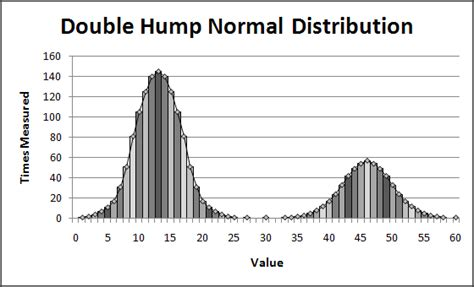
\includegraphics[scale=.7]{images/double_hump.jpg} \\

If we just told everyone that the arithmetic mean meant that it is the value that occurs the most, it would be confused as the mode, but if we told everyone it is a value that is probably somewhere in the middle, it would be confused as the median.

However, I will agree that in almost all stats courses, the interpretation of the maths is underemphasised and that students would have a much easier time learning what the maths means in words than just working with fancy symbols. My approach will be different from the book in that I will show you all these complicated looking mathematics, treat these fancy symbols as something like another language and translate them back into English, and hopefully when you think of stats in the future you can think about how the logic connects instead of just "well I've passed the t- or z-test, whatever that means, so my findings are correct". I hope that all my explanations will lay out clearly, both what the mathematical statements that we will learn mean, and also just as importantly (as we have seen the previous paragraphs), what they do not mean.

\hyperlink{https://en.wikipedia.org/wiki/Analysis_of_variance}{imp topic (anova)}

\section{Probability Theory}

\subsection{Set Theory}
\begin{defn}
    The set, $S$, of all possible outcomes of a particular experiment is called the \textit{sample space} for the experiment.
\end{defn}
\begin{defn}
    An \textit{event} is any collection of possible outcomes of an experiment, that is, any subset of $S$ (including $S$ itself).
\end{defn}
\begin{exmp} [Event operations]
    Selecting cards...
\end{exmp}
\begin{thm}
    \textit{For any three events, $A$, $B$, $C$, defined on a sample space $S$,}
    
    \textbf{a.} Commutativity
    \begin{align*}
        A \cup B = B \cup A, \\
        A \cap B = B \cap A;
    \end{align*}
    \textbf{b.} Associativity
    \begin{align*}
        A \cup (B \cup C) = (A \cup B) \cup C, \\
        A \cap (B \cap C) = (A \cap B) \cap C;
    \end{align*}
    \textbf{c.} Distributive Laws
    \begin{align*}
        A \cap (B \cup C) = (A \cap B) \cup (A \cap C), \\
        A \cup (B \cap C) = (A \cup B) \cap (A \cup C);
    \end{align*}
    \textbf{d.} DeMorgan's Laws
    \begin{align*}
        (A \cup B)^c = A^c \cap B^c, \\
        (A \cap B)^c = A^c \cup B^c.
    \end{align*}
\end{thm}
Proof can be done as an exercise
\begin{defn}
    Two events $A$ and $B$ are disjoint (or \textit{mutually exclusive}) if $A \cap B = \emptyset$. The events $A_1, A_2, ...$ are \textit{pairwise disojoint} (or \textit{mutually exclusive}) if $A_i \cap A_j = \emptyset$ for all $i \neq j$.
\end{defn}
\begin{defn}
    If $A_1, A_2, ...$ are pairwise disjoint and $\bigcup^\infty_{i = 0} A_i = S$, then the collection $A_1, A_2, ...$ forms a \textit{partition} of S.
\end{defn}

\subsubsection{Basics of probability Theory}

\begin{thm}
    If $P$ is a probability function and $A$ is any set in $S$, then

    \textbf{a.} $P(\emptyset) = 0$, where $\emptyset$ is the empty set; \\
    \textbf{b.} $P(A) \leq 1$; \\
    \textbf{c.} $P(A^c) = 1 - P(A)$.
\end{thm}
\begin{thm}
    If $P$ is a probability function and $A$ and $B$ are any sets in $\mathcal{B}$, then

    \textbf{a.} $P(B \cap A^c) = P(B) - P(A \cap B)$; \\
    \textbf{b.} $P(A \cup B) = P(A) + P(B) - P(A \cap B)$; \\
    \textbf{c.} If $A \subset B$, then $P(A) \leq P(B)$.
\end{thm}
\begin{thm}
    If a job consists of $k$ separate tasks, the $i$th of which can be done in $n_i$ ways, $i = 1, ..., k$, then the entire job can be done in $n_1 \times n_2 \times ... \times n_k$ ways.
\end{thm}
This is sometimes known as the Fundamental Theorem of Counting. The proof for this can be done as an exercise.
\begin{exmp}[Lottery - II]
    Although the Fundamental Theorem of Counting is a reasonable place to start...
\end{exmp}
\begin{defn}
    For a positive integer $n$, $n!$ (read $n$ factorial) is the product of all of the positive integers less than or equal to $n$. That is,
    \begin{align*}
        n! = n \times (n - 1) \times (n - 2) \times ... \times 3 \times 2 \times 1.
    \end{align*}
    Furthermore, we define $0! = 1$.
\end{defn}
\begin{defn}
    For nonnegative integers $n$ and $r$, where $n \geq r$, we define the symbol $\binom{n}{r}$, read $n$ \textit{choose} $r$, as
    \begin{align*}
        \binom{n}{r} = \frac{n!}{r!(n - r)!}
    \end{align*}
\end{defn}
\begin{center}
\begin{tabular}{c|c|c|}
     &  Without replacement & With replacement \\ \hline
     Ordered & $\frac{n!}{(n - r)!}$ & $n^r$ \\ 
     Unordered & $\binom{n}{r}$ & $\binom{n + r - 1}{r}$
\end{tabular}
\end{center}
\begin{exmp}[Poker]
    Consider choosing a five-card poker hand...
\end{exmp}
\begin{exmp}[Sampling with replacement]
    Consider sampling $r = 2$ items from $n = 3$ items...
\end{exmp}
 Some authors argue that it is appropriate to assign equal probabilities to the unordered outcomes when "randomly distributing $r$ indistinguishable balls into $n$ distinguishable urns." That is, an urn is chosen at random and a ball placed in it, and this is repeated $r$ times. The order in which the balls are placed is not recorded so, in the end, an outcome such as $\{1,3\}$ means one ball is in urn 1 and one ball is in urn 3. \\
 But here is the problem with this interpretation. Suppose two people observe this process, and Observer 1 will assign probability $\frac{2}{9}$ to the event $\{1,3\}$. Observer 2, who is observing exactly the same process, should also assign probability $\frac{2}{9}$ to this event. But if the six unordered outcomes are written on identical pieces of paper and one is randomly chosen to determine the placement of the balls, then the unordered outcomes each have probability $\frac{1}{6}$. So Observer 2 will assign probability $\frac{1}{6}$ to the event $\{1,3\}$. \\
 The confusion arises because the phrase "with replacement" will typically be interpreted with the sequential kinda of sampling we described above, leading to assigning a probability $\frac{2}{9}$ to the event $\{1,3\}$. This is the correct way to proceed, as probabilities should be determined by the sampling mechanism, not whether the balls are distinguishable or indistinguishable.
\begin{exmp}[Caldulating an average]
    An illustration of the distinguishable/indistinguishable approach... \\
    If there are $k$ places and we have $m$ different numbers repeated $k_1, k_2, ..., k_m$ times, then the number of ordered samples is $\frac{k!}{k_1!k_2!...k_m!}$. This type of counting is related to the \textit{multinomial distribution}, which we will see in Section 4.6. \\
    Figure 1.2.2 (p. 19 of book) is an elementary version of a very important statistical technique known as the \textit{bootstrap} (Efron and Tibshirani 1993). We will return to the bootstrap in Section 10.1.4
\end{exmp}
\subsubsection{Conditional Probability and Independence}

\begin{defn}
    \label{def 1.3.2}
    If $A$ and $B$ are events in $S$ and $P(B) > 0$, then the \textit{conditional probability} of $A$ \textit{given} $B$, written $P(A|B)$, is
    \begin{align*}
        P(A|B) = \frac{P(A \cap B)}{P(B)}
    \end{align*}
    Note that what happens in the conditional probability calculation is that $B$ becomes the sample space: $P(B|B) = 1$. The intuition is that our original sample space, $S$, has been updated to $B$. All further occurrences are then calibrated with respect to their relation to $B$. In particular, note what happens to conditional probabilities of disjoint sets. Suppose $A$ and $B$ are disjoint, so $P(A \cap B) = 0$. It then follows that $P(A|B) = P(B|A) = 0$.
\end{defn}

\begin{thm}[Bayes' Rule]
    Let $A_1, A_2, ...$ be a partition of the sample space, and let $B$ be any set. Then for each $i = 1, 2, ...$,
    \begin{align*}
        P(A_i|B) = \frac{P(B|A_i)P(A_i)}{\sum^\infty_{j = 1}P(B|A_j)P(A_j)}.
    \end{align*}
\end{thm}

\begin{defn}
    Two events, $A$ and $B$, are \textit{statistically independent} if
    \begin{align*}
        P(A \cap B) = P(A)P(B).
    \end{align*}
    Note that independence could have been equivalently defined by either $P(A|B) = P(A)$ or $P(B|A) = \frac{P(A|B)P(B)}{P(A)} = \frac{P(A)P(B)}{P(A)} = P(B)$. The advantage of defining it this way is that it treats the events symmetrically and will be easier to generalise to more than two events.
\end{defn}
\begin{thm}
    If $A$ and $B$ are independent events, then the following pairs are also independent:

    \textbf{a.} $A$ and $B^c$ \\
    \textbf{b.} $A^c$ and $B$ \\
    \textbf{c.} $A^c$ and $B^c$
\end{thm}
All three statements can be proved as an exercise.
\begin{defn}
    A collection of events $A_1, ..., A_n$ are \textit{mutually independent} if for any subcollection $A_{i_1}, ..., A_{i_k}$, we have
    \begin{align*}
        P(\bigcap^k_{j = 1} A_{i_j}) = \prod^k_{j = 1} P(A_{i_j}).
    \end{align*}
\end{defn}

\subsubsection{Random Variables}
\begin{defn}
    A \textit{random variable} is a function from a sample space $S$ into the real numbers.
\end{defn}

\subsubsection{Distribution Functions}
\begin{defn}
    The \textit{cumulative distribution function} or \textit{cdf} of a random variable $X$, denoted by $F_X(x)$, is defined by
    \begin{align*}
        F_X(x) = P_X(X \leq x),\ \forall x.
    \end{align*}
\end{defn}
\begin{thm}
    The function $F(x)$ is a cdf if and only if the following three conditions hold:

    \textbf{a.} $\lim_{x \rightarrow -\infty} F(x) = 0$ and $\lim_{x \rightarrow \infty} F(x) = 1$. \\
    \textbf{b.} $F(x)$ is a nondecreasing function of $x$. \\
    \textbf{c.} $F(x)$ is right-continuous; that is, for every number $x_0$, $\lim_{x \downarrow x_0} F(x) = F(x_0)$.
\end{thm}
Whether a cdf is continuous or has jumps corresponds to the associated random variable being continuous or not. In fact, the association is such that it is convenient to define continuous random variables in this way.
\begin{defn}
    A random variable $X$ is \textit{continuous} if $F_X(x)$ is a continuous function of $x$. A random variable is \textit{discrete} if $F_X(x)$ is a step function of $x$.
\end{defn}
\begin{defn}
    The random variables $X$ and $Y$ are \textit{identically distributed} if, for every set $A \in \mathcal{B}$, $P(X \in A) = P(Y \in A)$.
\end{defn}
\begin{thm}
    The following two statements are equivalent:

    \textbf{a.} The random variables $X$ and $Y$ are identically distributed. \\
    \textbf{b.} $F_X(x) = F_Y(x)$ for every $x$.
\end{thm}
Sufficiency can be proven as an exercise, necessity is very hard. See page 34.
\subsubsection{Density and Mass Functions}
Associated with a random variable $X$ and its cdf $F_X$ is another function, called either the probability density function (pdf) or probability mass function (pmf). The terms pdf and pmf refer, respectively, to the continuous and discrete cases. Both pdfs and pmfs are concerned with "point probabilities" of random variables.
\begin{defn}
    The \textit{probability mass function (pmf)} of a discrete random variable $X$ is given by
    \begin{align*}
        f_X(x) = P(X = x)\ \forall x.
    \end{align*}
\end{defn}
\begin{defn}
    The \textit{probability density function} or \textit{pdf}, $f_X(x)$, of a continuous random variable $X$ is the function that satisfies
    \begin{align*}
        F_X(x) = \int^x_{-\infty} f_X(t)\ dt\ \forall x.
    \end{align*}
\end{defn}
\begin{note}[notation]
    The expression "$X$ has a distribution given by $F_X(x)$" is abbreviated symbolically by "$X \sim F_X(x)$", where we read the symbol "$\sim$" as "is distributed as". We can similarly write $X \sim f_X(x)$ or, if $X$ and $Y$ have the same distribution, $X \sim Y$.
\end{note}
Since $P(X = x) = 0$ if $X$ is a continuous random variable,
\begin{align*}
    P(a < X < b) = P(a < X \leq b) = P(a \leq X < b) = P(a \leq X \leq b).
\end{align*}
It should be clear that the pdf (or pmf) contains the same information as the cdf and we should choose whichever one makes the problem simpler.
\begin{thm}
    A function $f_X(x)$ is a pdf (or pmf) of a random variable $X$ if and only if

    \textbf{a.} $f_X(x) \geq 0$ for all $x$. \\
    \textbf{b.} $\sum_x f_X(x) = 1$ (pmf) or $\int^\infty_{-\infty} f_X(x) dx = 1$ (pdf).
\end{thm}

\subsection{Expectation}

\subsubsection{Expectation of a Random Variable}

\begin{defn}
    The expected value, or mean, or first moment, of $X$ is defined to be
    \eqnum{
    \E{X} = \int x dF(x) = \begin{cases}
        \sum_{x} xf(x) & \text{If $X$ is discrete} \\
        \int xf(x) dx & \text{If $X$ is continuous}
    \end{cases}
    }
    assuming that the sum (or integral) is well defined. Use the following notation to denote the expected value of $X$
    \eqnum{
    \E{X} = \mathbb{E} X = \int x dF(x) = \mu = \mu_{X}.
    }
\end{defn}
$\int x dF(X)$ is used as a convenient unifying notation so we do not have to write $\sum_{x} xf(x)$ for discrete RVs and $\int xf(x) dx$ for continuous ones but be aware that $\int x dF(X)$ has a precise meaning that is discussed in real analysis course.

To ensure that $\E{X}$ is well defined, we say that $\E{X}$ exists if $\int_{x} \abs{x} dF_{X}(x) < \infty$. Otherwise, we say that the expectation does not exist.

To compute $\E{Y}$ when $Y = r(X)$, one way is to find $f_Y(y)$ then compute $\E{Y} = \int yf_{Y}(y) dy$.
\begin{thm}[The Rule of the Lazy Statistician]
    Let $Y = r(X)$. Then
    \eqnum{
    \E{Y} = \E{r(X)} = \int r(x) dF_{X}(x).
    }
\end{thm}
\eqnum{
Z = r(X,Y) \Rightarrow \E{Z} = \E{r(X,Y)} = \int \int r(x,y) dF(x,y).
}
The $k^{th}$ moment of $X$ is defined to be $\E{X^k}$ assuming that $\E{\abs{X}^k} < \infty$.
\begin{thm}
    If the $k^{th}$ moment exists and if $j < k$ then the $j^{th}$ moment exists.
\end{thm}
\begin{proof}
    \begin{align*}
        \E{\abs{X}^j} &= \int^{\infty}_{-\infty} \abs{x}^j f_{X}(x)\ dx \\
        &= \int_{\abs{x} \leq 1} \abs{x}^j f_{X}(x)\ dx + \int_{\abs{x} > 1} \abs{x}^j f_{X}(x)\ dx \\
        &\leq \int_{\abs{x} \leq 1} f_{X}(x)\ dx + \int_{\abs{x} > 1} \abs{x}^k f_{X}(x)\ dx \\
        &\leq 1 - \E{\abs{X}^k} < \infty.
    \end{align*}
\end{proof}
The $k^{th}$ central moment is defined to be $\E{(X - \mu)^k}$.

\subsubsection{Properties of Expectations}

\begin{thm}
    If $X_1, ..., X_n$ are RVs and $a_1, ..., a_n$ are constants, then
    \eqnum{
    \E{\sum_{i} a_i X_i} = \sum_i a_i \E{X_i}.
    }
\end{thm}
\begin{thm}
    Let $X_1, ..., X_n$ be independent RVs. Then
    \eqnum{
    \E{\prod^{n}_{i = 1} X_i} = \prod_i \E{X_i}.
    }
\end{thm}
Note the summation rule does not require independence but the product rule does.

\section{Statistical inference}

Statistical inference, or "learning" as it is called in comp sci, is the process of using data to infer the distribution that generated the data. A typical statistical inference question is \\

\textbf{Given a sample $X_1,...,X_n \sim F$, how do we infer $F$?}

\subsection{Parametric and Nonparametric Models}

A \textbf{statistical model} $\mathscr{F}$ is a set of distributions (or densities or regression functions). A \textbf{parametric model} is a set $\mathscr{F}$ that can be parameterized by a finite number of parameters. For example, assuming the data comes from a Normal distribution, the model is
\begin{align*}
    \mathscr{F} = \{f(x;\mu,\sigma) = \frac{1}{\sigma\sqrt{2\pi}} \exp{-\frac{1}{2\sigma^2}(x - \mu)^2},\ \mu \in \mathds{R}, \sigma > 0\}.
\end{align*}
This is a two-parameter model. Writing the density as $f(x;\mu,\sigma)$ shows that $x$ is a value of the RV while $\mu$ and $\sigma$ are parameters. In general, a parametric model takes the form
\begin{align*}
    \mathscr{F} = \{f(x;\theta):\theta \in \Theta\}
\end{align*}
where $\theta$ is an unknown parameter (or vector of parameters) that can take values in the \textbf{parameter space} $\Theta$. A \textbf{nonparametric model} is a set $\mathscr{F}$ that cannot be parameterized by a finite number of parameters. For example, $\mathscr{F}_{ALL} = \{\mathrm{all\ CDF's}\}$ is nonparametric\footnote{The distinction between parametric and nonparametric is more subtle than this but we don’t need a rigorous definition for our purposes}.

\begin{exmp}[Regression, prediction, and classification]
    Suppose we observe pairs of data $(X_1,Y_1),...,(X_n,Y_n)$. $X$ is called a predictor or regressor or feature or independent variable. $Y$ is called the outcome or the response variable or the dependent variable. We call $r(x) = \E{Y|X = x}$ the \textbf{regression function}. If we assume that $r \in \mathscr{F}$ where $\mathscr{F}$ is finite dimensional, then we have a \textbf{parametric regression model}. If $\mathscr{F}$ is not finite dimensional then we have a \textbf{nonparametric regression model}. The goal of predicting $Y$ for a new patient based on their $X$ value is called \textbf{prediction}. If $Y$ is discrete, then prediction is called \textbf{classification}. If we wish to estimate the function $r$, then we call this \textbf{regression} or \textbf{curve estimation}. Regression models are sometimes written as
    \eqnum{
    Y = r(X) + \epsilon
    }
    where $\E{\epsilon} = 0$. We can always rewrite a regression model this way. To see this, define $\epsilon = Y - r(X)$ and hence $Y = Y + r(X) - r(X) = r(X) + \epsilon$. Moreover, $\E{\epsilon} = \mathbb{E}\E{\epsilon|X} = \E{\E{Y - r(X)}|X} = \E{\E{Y|X} - r(X)} = \E{r(X) - r(X)} = 0$.
\end{exmp}

Notation: If $\mathscr{F} = \{f(x;\theta):\theta \in \Theta\}$ is a parametric model, we write $\mathds{P}_{\theta}(X \in A) = \int_{A}f(x;\theta) dx$ and $\mathbb{E}_{\theta}[r(X)] = \int r(x)f(x;\theta)dx$. The subscript $\theta$ indicates that the probability or expectation is w.r.t $f(x;\theta)$, not that we are averaging over $\theta$. Similarly, write $\mathbb{V}_{\theta}$ for the variance\footnote{There's no need to understand the logic behind the notation here, this is more for me so I don't lose track of what's happening}.

Most inferential problems can be divided into either estimation, confidence sets, or hypothesis testing. We are interested mainly in hypothesis testing so I will only provide a basic description of the other two.

\textbf{Point Estimation} \\
Point estimation refers to providing a single "best guess" of some quantity of interest. We denote a point estimate of $\theta$ by $\hat{\theta}$ or $\hat{\theta}_n$.

\textbf{Confidence Sets}\\
A $1 - \alpha$ \textbf{confidence interval} for a parameter $\theta$ is an interval $C_n = (a,b)$ where $a = a(X_1,...,X_n)$ and $b = b(X_1,...,X_n)$ are functions of the data such that
\begin{align}
    \mathds{P}_{\theta}(\theta \in C_n) \geq 1 - \alpha,\ \forall \theta \in \Theta.
\end{align}
In words, $(a,b)$ traps $\theta$ with probability $1 - \alpha$. We call $1 - \alpha$ the \textbf{coverage} of the confidence interval.

\textbf{Warning!} $C_n$ is random and $\theta$ is fixed. If $\theta$ is a vector then we use a \textbf{confidence set} instead of an interval.

\textbf{Interpretation:} Don't think of it as, if I repeat the experiment over and over, the interval will contain the parameter 95 percent of the time. This is correct but useless since experiments are rarely repeated that many times. A better interpretation is that if you construct 95 percent confidence intervals with many parameters (e.g. $\theta_1,\theta_2,\theta_3,...$) then 95 percent of the intervals you construct will trap the true parameter value.

\textbf{Note:} Remember that a confidfence interval is not a probability statement about $\theta$.

\textbf{Hypothesis Testing} \\
In hypothesis testing, we start with some default theory called a \textbf{null hypothesis} and ask if the data provides sufficient evidence to reject the theory. If not, we retain the null hypothesis.

\begin{exmp}[Test if a coin is fair]
    Let 
    \begin{align*}
        X_1,...,X_n \sim \mathrm{Bernoulli}(p)
    \end{align*}
    be $n$ independent coin flips. Suppose we want to test if the coin is fair. Let $H_0$ denote the hypothesis that the coin is fair and let $H_1$ denote the hypothesis. $H_0$ is called the \textbf{null hypothesis} and $H_1$ the \textbf{alternative hypothesis}. They can be written as
    \begin{align*}
        H_0:p = \frac{1}{2}\ \mathrm{versus}\ H_1:p \neq \frac{1}{2}.
    \end{align*}
    It seems reasonable to reject $H_0$ if $T = \abs{\hat{p}_n - \frac{1}{2}}$ is large. When we discuss hypothesis testing in detail, we will be more precise about how large $T$ should be to reject $H_0$.
\end{exmp}
Another question we could ask is if exposure to asbestos is associated with lung disease. We take some rats and randomly divide them into two groups. We expose one group to asbestos and leave the second group unexposed. Then we compare the disease rates in the two groups. Consider the following two hypotheses:

\textbf{The Null Hypothesis:} The disease rate is the same in the two groups. \\
\textbf{The Alternative Hypothesis:} The disease rate is not the same in the two groups.

If the exposed group has a much higher rate of disease than the unexposed group then we will reject the null hypothesis. This is an example of hypothesis testing. More formally, suppose that we partititon the parameter space $\Theta$ into two disjoint sets $\Theta_0$ and $\Theta_1$ and that we wish to test
\begin{align}
    H_0: \theta \in \Theta_0\ \text{ versus }\ H_1: \theta \in \Theta_1.
\end{align}
We call $H_0$ the null hypothesis and $H_1$ the alternative hypothesis.

Let $X$ be a random variable and let $\mathscr{X}$ be the range of $X$. We test a hypothesis by finding an appropriate subset of outcomes $R \subset \mathscr{X}$ called the rejection region. If $X \in R$ we reject the null hypothesis, otherwise, we do not reject the null hypothesis: \\
$X \in R \Rightarrow \text{ reject } H_0$ \\
$X \notin R \Rightarrow \text{ retain (do not reject) } H_0$.

Usually the rejection region $R$ is of the form
\begin{align}
    R = \{x: T(x) > c\}
\end{align}
where $T$ is a test statistic and $c$ is a critical value. The problem in hypothesis testing is to find an appropriate test statistic $T$ and an appropriate critical value $c$.

Hypothesis testing is like a legal trial. We assume someone is innocent unless the evidence strongly suggests that they are guilty. Similarly, we retain $H_0$ unless there is strong evidence to reject $H_0$. Rejecting $H_0$ when $H_0$ is true is called a type I error and retaining $H_0$ when $H_1$ is true is called a type II error.

\subsection{Hypothesis testing}

Summing up hypothesis testing. Every nonparametric procedure will have these steps.

\textit{First, state the hypotheses.} There are two types of hypotheses, null and alternate. The null hypothesis says that no difference exists between the conditions, groups, or variables. The alternate hypothesis, also called a research hypothesis, predicts a difference or relationship between conditions, groups, or variables.

The alternate hypothesis may be directional or nondirectional. A directional (one-tailed) hypothesis predicts a statistically significant change in a particular direction. A nondirectional (two-tailed) hypothesis predicts a statistically significant change, but in no particular direction.

\textit{We then set the risk (or level of significance) associated with the null hypothesis.} Whenever we perform a test, there is always some chance that the results we get are due to chance instead of any real difference. Therefore, when we perform such tests, we state the level of risk that we are willing to accept. The two types of errors we can make are type $I$, where we claim that there is a difference (alternate is true and null is false) when in reality there is no difference and the null hypothesis is true, and type $II$, where we claim there is no difference (null is true and alternate is false) when in reality there is a real difference and the null hypothesis is false. The commonly accepted way of stating your risk levels is in terms of the probability you allow yourself to make type $I$ errors $\alpha$. Most of the time, $\alpha = 0.05$ is used, which means that when we claim our alternate hypothesis is true, we are correct $95\%$ of the time.

\textit{We also choose a suitable test statistic based on the characteristics of the data.} For example, some tests are appropriate for two sample tests, while others are more appropriate for three or more samples. Different tests may also be suitable for different measurement scales. 

\textit{We then compute the test statistic.} This is usually done with a computer program and the interpretation is different for each statistic so there is not much to say here.

\textit{Determine what values the test statistic can take in order to reject the null hypothesis using the appropriate table of critical values for the particular statistic.} Finding this critical value may require you to use data characteristics such as the degrees of freedom, number of samples, and/or number of groups.

\textit{Compare test statistic value with critical value in the table. Interpret the results then report them.}

\section{Wilcoxon}

Imagine you give an attitude test to a small group of people. After you deliver some treatment, say a daily vitamin supplement for a few weeks, you give the same group of people another attitude test. You then compare the two measures to see if there is any meaningful difference between the two sets of scores.

The characteristic to note is that every test score is paired. Since everyone is tested twice, for each initial test score, there is another test score for that same person after the treatment. This forms a pair for each test score\footnote{Assuming no attrition, of course}. The parametric equivalent to these tests is called the Student's $t$-test, $t$-test for matched pairs, $t$-test for paired samples, or $t$-test for dependent samples.

Note that the procedures for the Wilcoxon signed-rank and sign tests change depending on whether the samples are small or large.

\subsection{Ranking Data}

Many nonparametric procedures involve ranking data values.
\begin{table}[h]
    \centering % Centers the table horizontally
    \begin{tabular}{|c|c|} % Defines a table with two centered columns, separated by vertical lines
        \hline % Draw a horizontal line
        Students who ate breakfast & Students who skipped breakfast \\ % Content of the first row separated by "&" symbol, ends with "\\" for a new row
        \hline
        \textbf{87} & 93 \\
        \hline
        \textbf{96} & 83 \\ 
        \hline
        \textbf{92} & 79 \\
        \hline
        \textbf{84} & 73 \\
        \hline
    \end{tabular}
    \caption{Healthy breakfast or not} % Adds a caption to the table
    \label{tab:breakfast} % Adds a label for referencing
\end{table}
To rank all values from the first table, we simply place them all in order in a new table from smallest to largest. The table below shows how to do this with our breakfast example, keeping the values for the students who ate breakfast bolded.
\begin{table}[h]
    \centering % Centers the table horizontally
    \begin{tabular}{|c|c|} % Defines a table with two centered columns, separated by vertical lines
        \hline % Draw a horizontal line
        Students who ate breakfast & Students who skipped breakfast \\ % Content of the first row separated by "&" symbol, ends with "\\" for a new row
        \hline
        73 & 1 \\
        \hline
        79 & 2 \\ 
        \hline
        83 & 3 \\
        \hline
        \textbf{84} & 4 \\
        \hline
        \textbf{87} & 5 \\
        \hline
        \textbf{92} & 6 \\
        93 & 7 \\
        \hline
        \textbf{96} & 8 \\
        \hline
    \end{tabular}
    \caption{Ranking data} % Adds a caption to the table
    \label{tab:ranked_breakfast} % Adds a label for referencing
\end{table}
On the surface, it seems that the students who ate breakfast scored higher. However, if you wish to claim statistical significance, some type of procedure or test is required.

What if we have ties? Imagine we replaced the score for the student with a rank of 4 (scoring 84 points) with 83 points. This student is now tied with the student with a rank of 3. We simply give the students the average of their rank values. See the table below for how this would work. The rows in bold are now the tied values instead of values for those who ate breakfast.
\begin{table}[h]
    \centering % Centers the table horizontally
    \begin{tabular}{|c|c|} % Defines a table with two centered columns, separated by vertical lines
        \hline % Draw a horizontal line
        Students who ate breakfast & Students who skipped breakfast \\ % Content of the first row separated by "&" symbol, ends with "\\" for a new row
        \hline
        73 & 1 \\
        \hline
        79 & 2 \\ 
        \hline
        \textbf{83} & \textbf{3.5} \\
        \hline
        \textbf{83} & \textbf{3.5} \\
        \hline
        87 & 5 \\
        \hline
        92 & 6 \\
        \hline
        93 & 7 \\
        \hline
        96 & 8 \\
        \hline
    \end{tabular}
    \caption{Ties in data} % Adds a caption to the table
    \label{tab:tied_breakfast} % Adds a label for referencing
\end{table}
Most nonparametric statistical tests require a different formula when a sample of data contains ties.

\subsection{Wilcoxon Signed-Rank/Wilcoxon Matched-Pairs}

The formula for computing the Wilcoxon $T$ for small samples is:
\begin{align}
    T = \text{smaller of } \sum\mathds{R}_{+}\ \text{and}\ \sum\mathds{R}_{-}
\end{align}
where $\sum\mathds{R}_{+}$ is the sum of the ranks with positive differences and $\sum\mathds{R}_{-}$ is the sum of the ranks with negative differences.

We then examine the $T$ statistic using the relevant table of critical values. However, if the number of pairs $n$ exceeds those available from the table, then a large sample approximation may be performed. Simply put, we compute a $z$-score and use a table with the normal distribution to obtain a critical region of $z$-scores. First calculate:
\begin{align}
    \Bar{x}_T = \frac{n(n + 1)}{4}
\end{align}
where $\Bar{x}_T$ is the mean and $n$ is the number of matched pairs included in the analysis,
\begin{align}
    s_T = \sqrt{\frac{n(n + 1)(2n + 1)}{24}}
\end{align}
where $s_T$ is the standard deviation. The $z$-score approximation is therefore:
\begin{align}
    z^{*} = \frac{T - \Bar{x}_T}{s_T}.
\end{align}

Let's work through a sample matched-pairs test with small data samples. The counseling staff of Clear Creek County School District has implemented a new program this year to attempt reducing bullying at primary schools. To evaluate the effectiveness of our anti-bullying program, the school district has decided to compare the percentage of successful interventions last year before the program began with the percentage of successful interventions this year with the program in place\footnote{You may realise that since we have not stated what kind of program this is nor defined clearly what "interventions" mean or what a "successful intervention" would look like, this is not a very good experiment. Hopefully in any experiments you run in real life, you will have defined criteria for success better than I have here but for now, we will assume that we have some well-defined concept of a "successful intervention".}. The next table shows 12 elementary school counselors and their reported percentage of successful interventions last year and this.
\begin{table}[h]
    \centering % Centers the table horizontally
    \begin{tabular}{|c|c|c|} % Defines a table with two centered columns, separated by vertical lines
        \hline % Draw a horizontal line
        Participant number & Last year & This year \\ % Content of the first row 
        \hline
        1 & 31 & 31 \\
        \hline
        2 & 14 & 14 \\ 
        \hline
        3 & 53 & 50 \\
        \hline
        4 & 18 & 30 \\
        \hline
        5 & 21 & 28 \\
        \hline
        6 & 44 & 48 \\
        \hline
        7 & 12 & 35 \\
        \hline
        8 & 36 & 32 \\
        \hline
        9 & 29 & 34 \\
        \hline
        10 & 29 & 34 \\
        \hline
        11 & 17 & 27 \\
        \hline
        12 & 40 & 42
    \end{tabular}
    \caption{Percentage of successful interventions} % Adds a caption to the table
    \label{tab:bullying} % Adds a label for referencing
\end{table}
Since the samples are small, we need a nonparametric procedure. Since we are comparing two related, or paired, samples, we will use the Wilcoxon matched-pairs test. We will use the steps laid out in the previous section.

\textit{State the null and alternative hypotheses.} The null hypothesis states that the counselors reported no difference in the percentages last year and this year. The alternative states that the counselors observed some differences between this year and last year. Note that our alternative hypothesis does not claim that these differences are supposed to be positive ones, so our alternative is a two-tailed, nondirectional hypothesis. They can be written as
\begin{align*}
    H_0:\mu_D = 0 \\
    H_A:\mu_D \neq 0.
\end{align*}
\textit{Set the level of risk.} It is standard to choose $\alpha = 0.05$, which states that we will make type $I$ errors $5\%$ of the time.

\textit{Choose the appropriate test statistic.} We have already shown that the Wilcoxon matched-pairs test is appropriate.

\textit{Compute the test statistic.} Exclude data points where the difference between two matched pairs is zero, then rank the data again using the \textbf{absolute values}. With the new ranks, check that the ranks with positive differences are $9,7,4.5,10,1,6,8,$ and $2$. Adding the ranks with positive difference we get $\sum\mathds{R}_{+} = 47.5$. The ranks with negative differences are $3$ and $4.5$, summing to $\sum\mathds{R}_{-} = 7.5$. We choose the smaller of the two rank sums and therefore the Wilcoxon is $T = 7.5$.

\textit{Determine the critical value needed to reject the null hypothesis.} To find the critical value of the Wilcoxon matched-pairs test, we need the sample size, level of significance, and type of hypothesis. Note that since we discarded the two participants with no reported differences between this year and the last, we now have a sample size of $10$ instead of $12$. The table in the course handbook says that for a significance level of $0.05$ with a two-tailed hypothesis and $n = 10$, the critical value is $T = 8$. An obtained value less than or equal to $8$ will lead us to reject our null hypothesis. 

\textit{Compare obtained value with critical value.} Since our obtained value $T = 7.5$ is less than the critical value, $8$, we reject the null hypothesis.

\textit{Interpret and report results.} By rejecting the null hypothesis, we suggest that a real difference exists between last year's percentages and this year's percentages. Reporting the results would go something like this. \\
For this experiment, the Wilcoxon signed rank (matched-pairs) test $(T = 7.5, n = 12, p < 0.05)$ indicated that the difference in percentage of successful interventions was statistically significant. In addition, the sum of the positive difference ranks ($\sum\mathds{R}_{+} = 47.5$ was larger than the sum of the negative difference ranks ($\sum\mathds{R}_{-} = 7.5$), showing a positive impact from the program. Therefore, our analysis supports that the new anti-bullying program provides positive benefits towards the improvement of the aspect of student behaviour that school counselors perceive.

\subsubsection{Confidence Intervals}

Now we aim to construct a confidence interval based on the Wilcoxon signed rank test for matched pairs. Such a confidence interval provides a range of values that fall within the population with a $100(1 - \alpha)$ percent chance. So now instead of just answering yes or no, we can say that the difference in successful interventions due to the new anti-bullying program is some interval $[x,y]$.

First, let us introduce ourselves with some notation. Index each participant as some $i = 1,\dots,n$. Each counselor $i$ has matched pair $(x_{1}^{i},x_{2}^{i})$, where $x_{1}^{i}$ is the $i$'s reported percentage of successful interventions before the anti-bullying program was implemented and $x_{2}^{i}$ the reported percentage after program implementation. Compute value $D_i = x_{1}^{i} - x_{2}^{i}$ for each participant $i$. Then compute $u_{ij}$ as defined below:
\begin{align*}
    u_{ij} = \frac{D_i + D_j}{2}\ \text{for all} 1 \leq i \leq j \leq n.
\end{align*}
So let's pause here to give some interpretation. All we have done here is said that the difference between the reported percentages of counselor $i$ is represented by $D_i$ so for each of our matched pair data points, we have another number $D_i$. Then we calculate $u_{ij}$ for all unique combinations of individuals. For example:
\begin{align*}
    u_{11} = \frac{D_1 + D_1}{2} = \frac{-3 + -3}{2} = -3 \\
    u_{12} = \frac{D_1 + D_2}{2} = \frac{-3 + 12}{2} = \frac{9}{2}.
\end{align*}
You may notice that the number of $u_{ij}$s we have is a counting problem. If you wish to practice, note that $u_{12} = u_{21}$ so we have an unordered problem with replacement. Then order these averages from smallest to largest. The median of the ordered averages gives a point estimate of the population median difference.

Use the table in the handbook to find the endpoints of the confidence interval. First, determine $T$ from the table that corresponds with the sample size and desired confidence such that $p = \alpha/2$. We seek to find a $95\%$ confidence interval and we have $n = 10$ and $p = 0.05/2$. For single-tailed hypotheses, the table provides $T = 8$. Note that we are using a single-tailed hypothesis because we wish to provide a confidence interval around the point estimate of the population median. Therefore, we construct two single-tailed hypotheses around the median with a level of significance that adds up to $\alpha = 0.05$.

The endpoints of the confidence interval are the $K$th smallest and $K$th largest values of $u_{ij}$, where $K = T + 1$. So for our case, $K = 9$. The ninth smallest value is $0.5$ and the ninth largest is $12$. Therefore, we can say that we are $95\%$ confident that the difference of successful interventions due to the new bullying programs lies between $0.5$ and $12$.

I can go through the same test with a large data sample and normal approximation if required.

\subsection{Wilcoxon Sign Test/Rank-Sum Test}

Related samples can be analyzed more efficiently if the data is reduced to, or already comes in, dichotomous (binary) results. This method is based on Gibbons and Chakraborti (2010).

We start by identifying the sign of the difference demonstrated by each set from the related data samples, then sum all positive and negative differences as $n_p$ and $n_n$, respectively. 



\end{document}